\documentclass[12pt,a4paper,onecolumn]{exam}
\usepackage{amsmath}
\usepackage{amssymb}
\usepackage{graphicx}
\usepackage{float}
\usepackage{geometry}
\usepackage{tikz}
\usepackage[skins]{tcolorbox} % Use [skins] to get the rounded shape


% --- Define our simple \questionheader command ---
\newcommand{\questionheader}[1]{%
  \begin{tcolorbox}[
    enhanced,
    colback=black,
    coltext=white,
    boxrule=0pt,
    fontupper=\Large\bfseries,
    arc=4mm
  ]
  #1
  \end{tcolorbox}%
}
% --- End of definition ---
\newtcolorbox{answerbox}[1]{
  boxrule=0.4pt,   % Sets the thickness of the border
  colback=white,   % Sets the background color
  height=#1,       % <-- Use the first argument (#1) as the height
}


\usepackage[font = small]{caption}
\usepackage{subcaption}

\newenvironment{blanksolution}
  {%
    \renewcommand{\solutiontitle}{\noindent}%
    \begin{solution}%
  }%
  {\end{solution}}
\usepackage{listings}

\lstset{
    language=Python,
    basicstyle=\ttfamily,
    }

\pagestyle{headandfoot}
% \firstpageheader{Assignment 2}{}{Dwaipayan Haldar}
\runningheader{Assignment 1}{Detection and Estimation Theory}{Dwaipayan Haldar}


\begin{document}

\begingroup
    \centering
    \LARGE E1 244 Detection and Estimation Theory\\
    \LARGE Assignment 1\\[0.5em]
    \large Dwaipayan Haldar\par
    \large \today\\[0.5em] 
\endgroup
\noindent\rule{\textwidth}{0.5pt}
\printanswers
\renewcommand{\solutiontitle}{\noindent\textbf{Ans:}\enspace}

\questionheader{Problem 1 (6.3)}

\begin{solution}
The shifted exponential distribution is given by:
\[
f(x|\mu, \sigma) = \frac{1}{\sigma} e^{-\frac{(x-\mu)}{\sigma}}, \quad \mu < x < \infty, \quad 0 < \sigma < \infty
\]
This can be written as:
\[
f(x|\mu, \sigma) = \frac{1}{\sigma} e^{-\frac{(x-\mu)}{\sigma}} \cdot \mathbf{1}\{\mu < x < \infty\}
\]

Let $\mathbf{X} = (X_1, X_2, \ldots, X_n)$ and $\boldsymbol{\theta} = \begin{bmatrix} \mu \\ \sigma \end{bmatrix}$.

The joint pdf is:
\begin{align*}
P_{\theta}(\mathbf{X}) &= \prod_{i=1}^{n} f(x = X_i | \mu, \sigma) \\
&= \frac{1}{\sigma^n} \prod_{i=1}^{n} e^{-\frac{(X_i - \mu)}{\sigma}} \cdot \mathbf{1}\{\mu < X_i < \infty\} \\
&= \frac{1}{\sigma^n} e^{-\frac{(\sum X_i - n\mu)}{\sigma}} \cdot \mathbf{1}\{\mu < \min_i(X_i) < \infty\}
\end{align*}

By the \textbf{Neyman-Fisher Factorization Theorem}:

If $P_{\theta}(\mathbf{X}) = g(T(\mathbf{X}), \boldsymbol{\theta}) \cdot h(\mathbf{X})$, then $T(\mathbf{X})$ is a sufficient statistic for $\boldsymbol{\theta}$.

Here, we can identify:
\[
g(T(\mathbf{X}), \boldsymbol{\theta}) = \frac{1}{\sigma^n} e^{-\frac{(\sum X_i - n\mu)}{\sigma}} \cdot \mathbf{1}\{\mu < \min_i(X_i) < \infty\}
\]
and
\[
h(\mathbf{X}) = 1
\]

Therefore, the \textbf{sufficient statistic} is:
\[
\boxed{T(\mathbf{X}) = \begin{bmatrix} \min_i(X_i) \\ \sum_i X_i \end{bmatrix}}
\]
\end{solution}

\questionheader{Problem 2 (6.9)}

\begin{solution}
\textbf{(a)} The pdf is:
\[
f(x|\theta) = \frac{1}{\sqrt{2\pi}} e^{-\frac{(x-\theta)^2}{2}}
\]

Let $\mathbf{X} = (X_1, X_2, \ldots, X_n)$ and $\mathbf{Y} = (Y_1, Y_2, \ldots, Y_n)$ be two data points.

\begin{align*}
P_{\theta}(\mathbf{X}) &= \prod_{i=1}^{n} f(x = X_i | \theta) = \prod_{i=1}^{n} \frac{1}{\sqrt{2\pi}} e^{-\frac{(X_i - \theta)^2}{2}} \\
&= \frac{1}{(2\pi)^{n/2}} e^{-\frac{n}{2}(\bar{X} - \theta)^2} \cdot e^{-\frac{1}{2}\sum(X_i - \bar{X})^2}
\end{align*}

Similarly:
\[
P_{\theta}(\mathbf{Y}) = \frac{1}{(2\pi)^{n/2}} e^{-\frac{n}{2}(\bar{Y} - \theta)^2} \cdot e^{-\frac{1}{2}\sum(Y_i - \bar{Y})^2}
\]

The likelihood ratio is:
\begin{align*}
\frac{P_{\theta}(\mathbf{X})}{P_{\theta}(\mathbf{Y})} &= e^{-\frac{n}{2}[(\bar{X}-\theta)^2 - (\bar{Y}-\theta)^2]} \cdot e^{-\frac{1}{2}[\sum(X_i-\bar{X})^2 - \sum(Y_i-\bar{Y})^2]} \\
&= e^{-\frac{n}{2}[\bar{X}^2 - \bar{Y}^2 - 2\theta(\bar{X}-\bar{Y})]} \cdot e^{-\frac{1}{2}[\sum(X_i-\bar{X})^2 - \sum(Y_i-\bar{Y})^2]}
\end{align*}

If this is a constant function of $\theta$, then:
\[
\Rightarrow 2\theta(\bar{X} - \bar{Y}) = 0 
\]
\[
\Rightarrow \bar{X} - \bar{Y} = 0 \Rightarrow \bar{X} = \bar{Y}
\]

And if $\bar{X} = \bar{Y}$, then:
\[
\frac{P_{\theta}(\mathbf{X})}{P_{\theta}(\mathbf{Y})} = e^{-\frac{1}{2}[\sum(X_i-\bar{X})^2 - \sum(Y_i-\bar{Y})^2]}
\]
which is a constant function of $\theta$.

So, $\boxed{\bar{X}}$ \textbf{is a minimal sufficient statistic for} $\theta$.

\vspace{1em}
\textbf{(d)} Let $\mathbf{X} = (X_1, X_2, \ldots, X_n)$ and $\mathbf{Y} = (Y_1, Y_2, \ldots, Y_n)$ be two random samples.

Then:
\[
P_{\theta}(\mathbf{X}) = \prod_{i=1}^{n} f(x = X_i | \theta) = \prod_{i=1}^{n} \frac{1}{\pi[1 + (X_i - \theta)^2]} = \frac{1}{\pi^n} \cdot \frac{1}{\prod_{i=1}^{n}(1 + (X_i - \theta)^2)}
\]

Similarly:
\[
P_{\theta}(\mathbf{Y}) = \frac{1}{\pi^n} \cdot \frac{1}{\prod_{i=1}^{n}(1 + (Y_i - \theta)^2)}
\]

So:
\[
\frac{P_{\theta}(\mathbf{X})}{P_{\theta}(\mathbf{Y})} = \frac{\prod_{i=1}^{n}(1 + (Y_i - \theta)^2)}{\prod_{i=1}^{n}(1 + (X_i - \theta)^2)}
\]

The numerator and denominator are functions of $\theta$. If $\frac{P_{\theta}(\mathbf{X})}{P_{\theta}(\mathbf{Y})}$ is independent of $\theta$, then all the coefficients in the numerator and denominator must be the same.
\[
\Rightarrow X_i = Y_i \quad \forall i = 1, 2, \ldots, n
\]

And if $X_i = Y_i$ $\forall i = 1, 2, \ldots, n$, then $\frac{P_{\theta}(\mathbf{X})}{P_{\theta}(\mathbf{Y})}$ is independent of $\theta$.

So, $\boxed{T(\mathbf{X}) = (X_1, X_2, \ldots, X_n)}$ \textbf{is the minimal sufficient statistic for} $\theta$.

\vspace{1em}
\textbf{(e)} Let $\mathbf{X} = (X_1, X_2, \ldots, X_n)$ and $\mathbf{Y} = (Y_1, Y_2, \ldots, Y_n)$ be two random samples.

\[
P_{\theta}(\mathbf{X}) = \prod_{i=1}^{n} f(x = X_i | \theta) = \frac{1}{2^n} e^{-\sum_i |X_i - \theta|}
\]

Similarly:
\[
P_{\theta}(\mathbf{Y}) = \frac{1}{2^n} e^{-\sum_i |Y_i - \theta|}
\]

\[
\frac{P_{\theta}(\mathbf{X})}{P_{\theta}(\mathbf{Y})} = e^{-\sum_i \{|X_i - \theta| - |Y_i - \theta|\}}
\]

This term will be independent of $\theta$ only when:
\[
\text{number of } X_i < \theta = \text{number of } Y_i < \theta \quad \forall \theta \in \Theta
\]

It is only possible when $X_{(i)} = Y_{(i)}$, i.e., the order statistics are the same.

The reverse side: $X_{(i)} = Y_{(i)} \Rightarrow e^{-\sum_i \{|X_i - \theta| - |Y_i - \theta|\}}$ is independent of $\theta$ (trivial).

So, $\boxed{T(\mathbf{X}) = \{X_{(1)}, X_{(2)}, \ldots, X_{(n)}\}}$ \textbf{is the minimal sufficient statistic}.
\end{solution}

\questionheader{Problem 3 (6.12)}

\begin{solution}
\textbf{(a)} Given $P_{\theta}(X | N = n) = \binom{n}{X} \theta^X (1-\theta)^{n-X}$

For another observation $(Y, M)$, we get the distribution as:
\[
P_{\theta}(Y | M = m) = \binom{m}{Y} \theta^Y (1-\theta)^{m-Y}
\]

\[
\frac{P_{\theta}(X | N = n)}{P_{\theta}(Y | M = m)} = \frac{\binom{n}{X}}{\binom{m}{Y}} \cdot \frac{\theta^X (1-\theta)^{n-X}}{\theta^Y (1-\theta)^{m-Y}}
\]

This is independent of $\theta$ only when $m = n$ and $X = Y$.

Reverse is trivially true.

So, $\boxed{(X, N)}$ \textbf{is the minimal sufficient statistic}.

Distribution of $N$ is fixed. So $N$ is \textbf{ancillary} for $\theta$.

\vspace{1em}
\textbf{(b)} $P_{\theta}(X, N) = P_{\theta}(X|N) \cdot P_{\theta}(N) = \binom{N}{X} \theta^X (1-\theta)^{N-X} \cdot p_N$

Now:
\begin{align*}
E_{\theta}\left(\frac{X}{N}\right) &= \sum_{N \geq 1} \sum_{X=0}^{N} \frac{X}{N} \cdot \binom{N}{X} \theta^X (1-\theta)^{N-X} \cdot p_N \\
&= \sum_{N \geq 1} \frac{p_N}{N} \cdot \sum_{X=1}^{N} X \cdot \frac{N!}{X!(N-X)!} \cdot \theta^X (1-\theta)^{N-X} \\
&= \sum_{N \geq 1} \frac{p_N}{N} \cdot \sum_{X=1}^{N} N \cdot \binom{N-1}{X-1} \cdot \theta^X (1-\theta)^{N-X} \\
&= \sum_{N \geq 1} \frac{p_N}{N} \cdot N \cdot \theta \cdot \sum_{X=1}^{N} \binom{N-1}{X-1} \cdot \theta^{X-1} (1-\theta)^{N-X}
\end{align*}

Define $Y = X - 1$, then:
\begin{align*}
E_{\theta}\left(\frac{X}{N}\right) &= \sum_{N \geq 1} p_N \cdot \theta \cdot \sum_{Y=0}^{N-1} \binom{N-1}{Y} \cdot \theta^Y (1-\theta)^{N-1-Y} \\
&= \sum_{N \geq 1} p_N \cdot \theta = \theta \cdot \sum_{N \geq 1} p_N = \theta
\end{align*}

So, $\boxed{\frac{X}{N}}$ \textbf{is the unbiased estimator of} $\theta$.

\vspace{1em}
\textbf{(c)} $\text{Var}\left(\frac{X}{N}\right) = E\left(\frac{X}{N}\right)^2 - \left[E\left(\frac{X}{N}\right)\right]^2$

Now, $E\left(\frac{X^2}{N^2}\right) = E\left(\frac{X(X-1)}{N^2} + \frac{X}{N^2}\right)$

\begin{align*}
E\left(\frac{X(X-1)}{N^2}\right) &= \sum_{N \geq 1} \frac{p_N}{N^2} \cdot \sum_{X=2}^{N} X(X-1) \cdot \frac{N!}{X!(N-X)!} \cdot \theta^X (1-\theta)^{N-X} \\
&= \sum_{N \geq 1} \frac{p_N}{N^2} \cdot N(N-1) \cdot \theta^2 \cdot \sum_{X=2}^{N} \binom{N-2}{X-2} \cdot \theta^{X-2} (1-\theta)^{N-X} \\
&= \theta^2 \sum_{N \geq 1} \frac{p_N}{N^2} \cdot N(N-1) \cdot (\theta + 1 - \theta)^{N-2} \quad \text{[By similar substitution]} \\
&= \theta^2 \sum_{N \geq 1} \frac{p_N (N-1)}{N}
\end{align*}

Similarly, $E\left(\frac{X}{N^2}\right) = \theta \sum_{N \geq 1} \frac{p_N}{N}$

So, $E\left(\frac{X^2}{N^2}\right) = \sum_{N \geq 1} \frac{p_N}{N} \left[\theta^2(N-1) + \theta\right]$

Now:
\begin{align*}
\text{Var}\left(\frac{X}{N}\right) &= \sum_{N \geq 1} \frac{p_N}{N} \left[\theta^2(N-1) + \theta\right] - \theta^2 \\
&= \sum_{N \geq 1} \frac{p_N}{N} \left[\theta^2(N-1) + \theta\right] - \theta^2 \sum_{N \geq 1} \frac{p_N \cdot N}{N} \\
&= \sum_{N \geq 1} \frac{p_N}{N} \left[\theta - \theta^2\right] = \theta(1-\theta) \sum_{N \geq 1} \frac{p_N}{N}
\end{align*}

\[
\boxed{\text{Var}\left(\frac{X}{N}\right) = \theta(1-\theta) \cdot E\left(\frac{1}{N}\right)}
\]
\end{solution}

\questionheader{Problem 4 (6.18)}

\begin{solution}
Let $Y = X_1 + X_2 + \cdots + X_n$ where $X_i \sim \text{Poisson}(\lambda)$ i.i.d.

\[
P(X_i = x) = \frac{\lambda^x e^{-\lambda}}{x!}, \quad x = 0, 1, 2, \ldots
\]

The moment generating function of $X_i$ is:
\begin{align*}
M_X(t) = E(e^{tX}) &= \sum_{x \geq 0} e^{tx} \cdot \frac{\lambda^x e^{-\lambda}}{x!} \\
&= \sum_{x \geq 0} \frac{(\lambda e^t)^x \cdot e^{-\lambda}}{x!} \\
&= e^{-\lambda} \sum_{x \geq 0} \frac{(\lambda e^t)^x}{x!} \\
&= e^{-\lambda} \cdot e^{\lambda e^t} = e^{\lambda(e^t - 1)}
\end{align*}

\begin{align*}
M_Y(t) = E(e^{tY}) &= E(e^{t(X_1 + X_2 + \cdots + X_n)}) \\
&= E(e^{tX_1}) \cdot E(e^{tX_2}) \cdots E(e^{tX_n}) \\
&= e^{\lambda(e^t - 1)} \cdot e^{\lambda(e^t - 1)} \cdots e^{\lambda(e^t - 1)} \\
&= e^{n\lambda(e^t - 1)}
\end{align*}

So, $Y \sim \text{Poisson}(n\lambda)$.

Therefore, $T = \sum_i X_i \sim \text{Poisson}(n\lambda)$.

Now, if $E_{\lambda}(g(T)) = 0$ $\forall \lambda$:
\begin{align*}
E_{\lambda}(g(T)) &= \sum_{t=0}^{\infty} g(t) \cdot \frac{(n\lambda)^t \cdot e^{-n\lambda}}{t!} = 0 \quad \forall \lambda \\
&= e^{-n\lambda} \sum_{t=0}^{\infty} \frac{g(t) \cdot (n\lambda)^t}{t!} = 0 \quad \forall \lambda
\end{align*}

Let $\frac{g(t) \cdot n^t}{t!} = \alpha(t)$.

So, $\sum_{t=0}^{\infty} \alpha(t) \cdot \lambda^t = 0 \quad \forall \lambda$

Since it is a polynomial in $\lambda$, all coefficients must be 0.
\[
\Rightarrow \alpha(t) = 0 \Rightarrow g(t) = 0 \quad \forall t
\]

\textbf{So, the family of distribution of $\sum X_i$ is complete.}
\end{solution}

\questionheader{Problem 5 (6.19)}

\begin{solution}
\textbf{Distribution 1:}

Let $T \sim \text{Dist 1}$, i.e., $P(T=0) = p$, $P(T=1) = 3p$, $P(T=2) = 1-4p$ for $0 < p < 1/4$.

If $E_p(g(T)) = g(0) \cdot p + g(1) \cdot 3p + g(2) \cdot (1-4p) = 0$
\[
= \{g(0) + 3g(1) - 4g(2)\} \cdot p + g(2) = 0
\]

We can find $g(0) = 1$, $g(1) = -\frac{1}{3}$, $g(2) = 0$ for all $0 < p < 1/4$.

In that case $\forall p$: $E_p(g(T)) = 0$ but $g(T) \neq 0$ $\forall t$.

\textbf{So, Distribution 1 is NOT complete.}

\vspace{1em}
\textbf{Distribution 2:}

Let $T \sim \text{Dist 2}$, i.e., $P(T=0) = p$, $P(T=1) = p^2$, $P(T=2) = 1-p-p^2$ for $0 < p < 1/2$.

If $E_p(g(T)) = g(0) \cdot p + g(1) \cdot p^2 + (1-p-p^2) \cdot g(2) = 0$
\[
g(2) + \{g(0) - g(2)\} \cdot p + \{g(1) - g(2)\} \cdot p^2 = 0
\]

All the coefficients must be 0 for all $0 < p < 1/2$:
\begin{align*}
g(2) &= 0 \\
g(0) - g(2) &= 0 \\
g(1) - g(2) &= 0
\end{align*}
\[
\Rightarrow g(0) = 0, \quad g(1) = 0, \quad g(2) = 0
\]

\textbf{So, Distribution 2 family of $X$ is complete.}
\end{solution}

\questionheader{Problem 6 (6.30)}

\begin{solution}
\textbf{(a)} Let $X_{(1)} = \min_i X_i$ and $\mathbf{X} = (X_1, X_2, \ldots, X_n)$.

\begin{align*}
P_{\theta}(\mathbf{X}) &= \prod_{i=1}^{n} f(x = X_i | \mu) \\
&= \prod_{i=1}^{n} e^{-(X_i - \mu)} \cdot \mathbf{1}\{\mu < X_i\} \\
&= e^{-(\sum X_i - n\mu)} \cdot \mathbf{1}\{\mu < \min_i(X_i)\} \\
&= \underbrace{e^{-\sum X_i}}_{h(\mathbf{X})} \cdot \underbrace{e^{n\mu} \cdot \mathbf{1}\{\mu < X_{(1)}\}}_{g(T(\mathbf{X}), \theta)}
\end{align*}

So, by \textbf{Neyman-Fisher Factorization}:

$T(\mathbf{X}) = X_{(1)}$ is a \textbf{sufficient statistic}.

\vspace{0.5em}
\textbf{Finding the distribution of $X_{(1)}$:}

$X_{(1)} = \min\{X_1, X_2, \ldots, X_n\}$

\begin{align*}
P(X_{(1)} < t) &= 1 - P(X_{(1)} > t) \\
&= 1 - P(\min_i\{X_i\} > t) \\
&= 1 - P(X_1 > t) \cdot P(X_2 > t) \cdots P(X_n > t)
\end{align*}

Now:
\begin{align*}
P(X_i < t) &= \int_{-\infty}^{t} e^{-(x-\mu)} \cdot \mathbf{1}\{\mu < x\} dx = \int_{\mu}^{t} e^{-(x-\mu)} dx \\
&= \int_{0}^{t-\mu} e^{-y} dy \quad [\text{taking } y = x - \mu] \\
&= \left[-e^{-y}\right]_0^{t-\mu} = 1 - e^{-(t-\mu)}, \quad t > \mu
\end{align*}

Therefore:
\[
P(X_{(1)} < t) = 1 - e^{-(t-\mu)n}, \quad t > \mu
\]

The pdf is:
\[
p_{\mu}(X_{(1)}) = \frac{d}{dt}\left\{1 - e^{-(t-\mu)n}\right\} = n \cdot e^{\mu n} \cdot e^{-nt} = n \cdot e^{-(t-\mu)n}, \quad t > \mu
\]

\textbf{Proving completeness:}

Now, if $E_{\mu}(g(T)) = 0$ $\forall \mu \in \mathbb{R}$:
\begin{align*}
E_{\mu}(g(T)) &= \int_{-\infty}^{\infty} g(t) \cdot n \cdot e^{-(t-\mu)n} \cdot \mathbf{1}\{t > \mu\} dt \\
&= \int_{\mu}^{\infty} g(t) \cdot n \cdot e^{-(t-\mu)n} dt = 0 \quad \forall \mu \in \mathbb{R}
\end{align*}

Take $u = t - \mu$:
\[
\Rightarrow \int_{0}^{\infty} g(u + \mu) \cdot n \cdot e^{-nu} du = 0
\]

$\Rightarrow$ Convolution with exponential kernel is 0.

$\Rightarrow g$ is zero $\forall t$.

$\Rightarrow$ \textbf{$X_{(1)}$ is a complete statistic.}

\vspace{1em}
\textbf{(b)} Let $Y \sim \exp(1)$, i.e., $f(y) = e^{-y}$, $0 < y < \infty$.

Now, $X = Y + \mu$ (shifted by constant $\mu$).

\[
S^2 = \frac{1}{n-1} \sum (X_i - \bar{X})^2 = \frac{1}{n-1} \sum (Y_i - \bar{Y})^2
\]

Note that $\sum (Y_i - \bar{Y})^2$ does not depend on $\mu$.

So, $S^2$ is an \textbf{ancillary statistic}.

So, by \textbf{Basu's Theorem}: $\boxed{X_{(1)} \text{ and } S^2 \text{ are independent}}$.
\end{solution}

\questionheader{Problem 7 (6.34)}

\begin{solution}
\textbf{Experiment 1:} $N$ chosen randomly, then $N$ Bernoulli trials were done.

\textbf{Experiment 2:} $N$ is fixed at $n$.

Sample space: $\mathcal{Y}_1 = \{0, 1, 2, \ldots\}$, $\mathcal{Y}_2 = \{0, 1, 2, \ldots, n\}$

\vspace{0.5em}
For Experiment 1:
\[
P_{\theta}^{(1)}(X, N) = p_N \cdot \binom{N}{X} \theta^X (1-\theta)^{N-X}
\]

For Experiment 2:
\[
P_{\theta}^{(2)}(X) = \binom{n}{X} \theta^X (1-\theta)^{n-X}
\]

For $N = n$:
\[
P_{\theta}^{(1)}(X, N = n) = p_n \cdot \binom{n}{X} \theta^X (1-\theta)^{n-X} \propto P_{\theta}^{(2)}(X)
\]

\textbf{So, the likelihood is the same (up to a constant that doesn't depend on $\theta$).}

\textbf{Therefore, if $N$ is chosen to be $n$, it does not matter whether it was chosen randomly or not.} The inference about $\theta$ based on the likelihood will be identical in both cases.
\end{solution}

\questionheader{Problem 8}

\begin{solution}
Let $y_k \sim \text{i.i.d. Unif}(0, \theta)$ for $k = 1, 2, \ldots, N$.

Consider the two estimates:
\[
\hat{\theta}_1 = \max_{k=1}^{N}\{y_k\} \quad \text{and} \quad \hat{\theta}_2 = \frac{2}{N} \sum_{k=1}^{N} y_k
\]

\textbf{(a)} For $N = 10,000$ and $\theta = 1, 2, 3, 4$:

\begin{figure}[H]
    \centering
    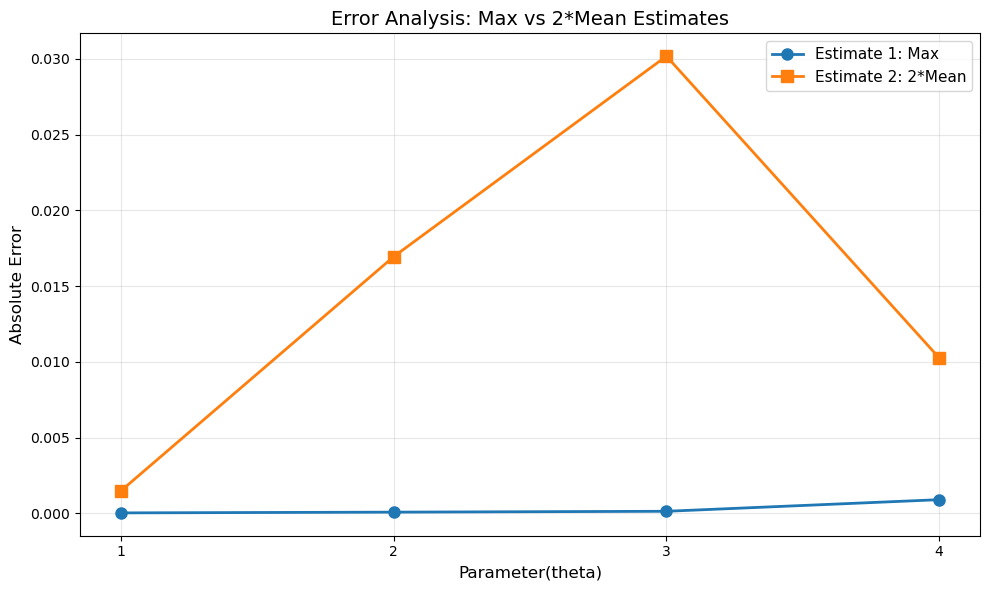
\includegraphics[width=0.8\textwidth]{P08a.png}
    \caption{Estimation error comparison for $\hat{\theta}_1$ (Max) and $\hat{\theta}_2$ (2$\times$Mean)}
\end{figure}

\textbf{Discussion:} The Max estimator ($\hat{\theta}_1$) performs better than the $2 \times$Mean estimator ($\hat{\theta}_2$) for all values of $\theta$. This was obvious as discussed in the class, the max estimator is a sufficient statistics while the twice of mean statistics is not. And sufficient statistics captures all the information effectively giving better estimation than a not sufficient statistics. 
\phantom{123}\\


\textbf{(b)} For $\theta = 1$ and $N = 10, 50, 100, 1000, 5000, 10000$:

\begin{figure}[H]
    \centering
    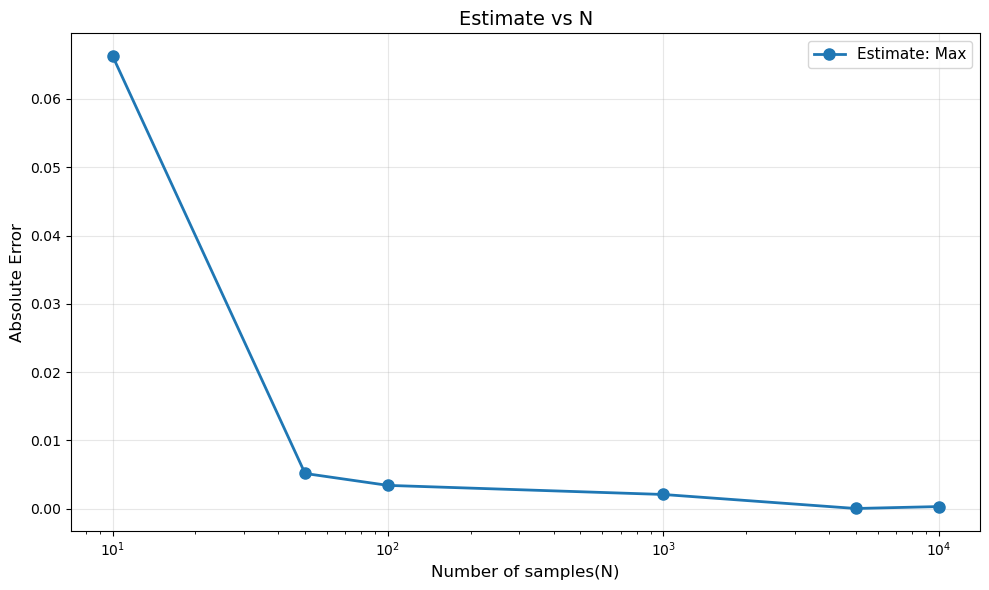
\includegraphics[width=0.8\textwidth]{P08b.png}
    \caption{Estimation error of $\hat{\theta}_1$ (Max) as a function of $N$}
\end{figure}

\textbf{Discussion:} The estimation error decreases as $N$ increases, showing a roughly linear trend on the semi-log plot. This is the golden rule of statistics. The idea mainly shown here is statistical regularity. As we increase the number of samples, the error of good estimator will converge to 0. Already, it is shown in the earlier problem that the max is a good estimator. 
\end{solution}




\end{document}
